\chapter{Experiments}
\section{Dropout Experiment}

\begin{figure}[ht]
   \centering
   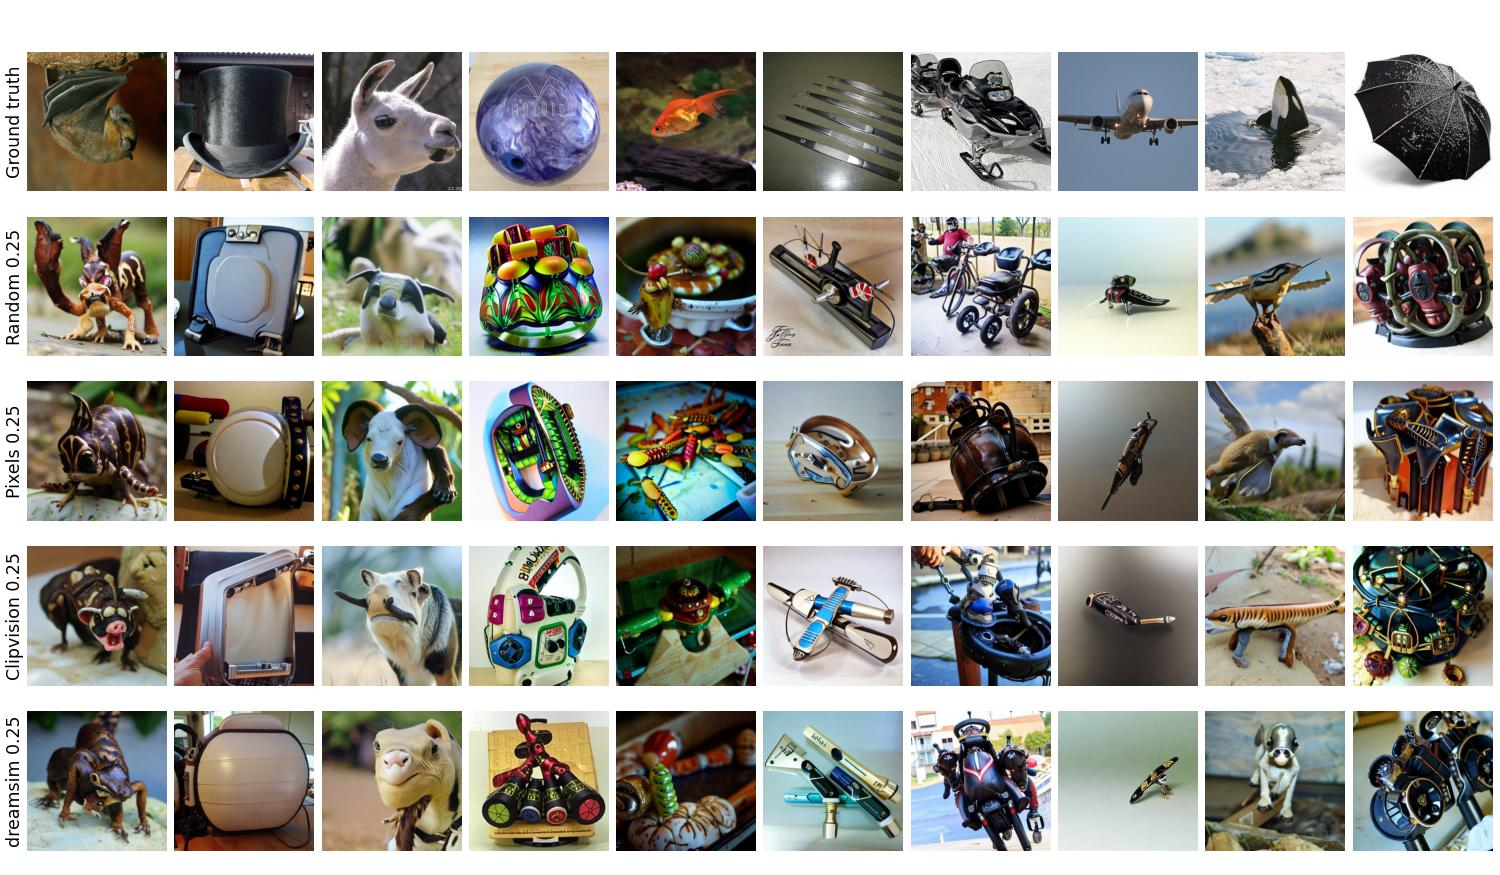
\includegraphics[width=1\textwidth]{plots/dropout_qual_eval_bd_test.JPEG}
   \caption{Qualitative Results for different dropout strategies with the brain-diffuser on natural test images}\label{fig:dropout_qual_eval_bd_test}
\end{figure}

\begin{figure}[ht]
   \centering
   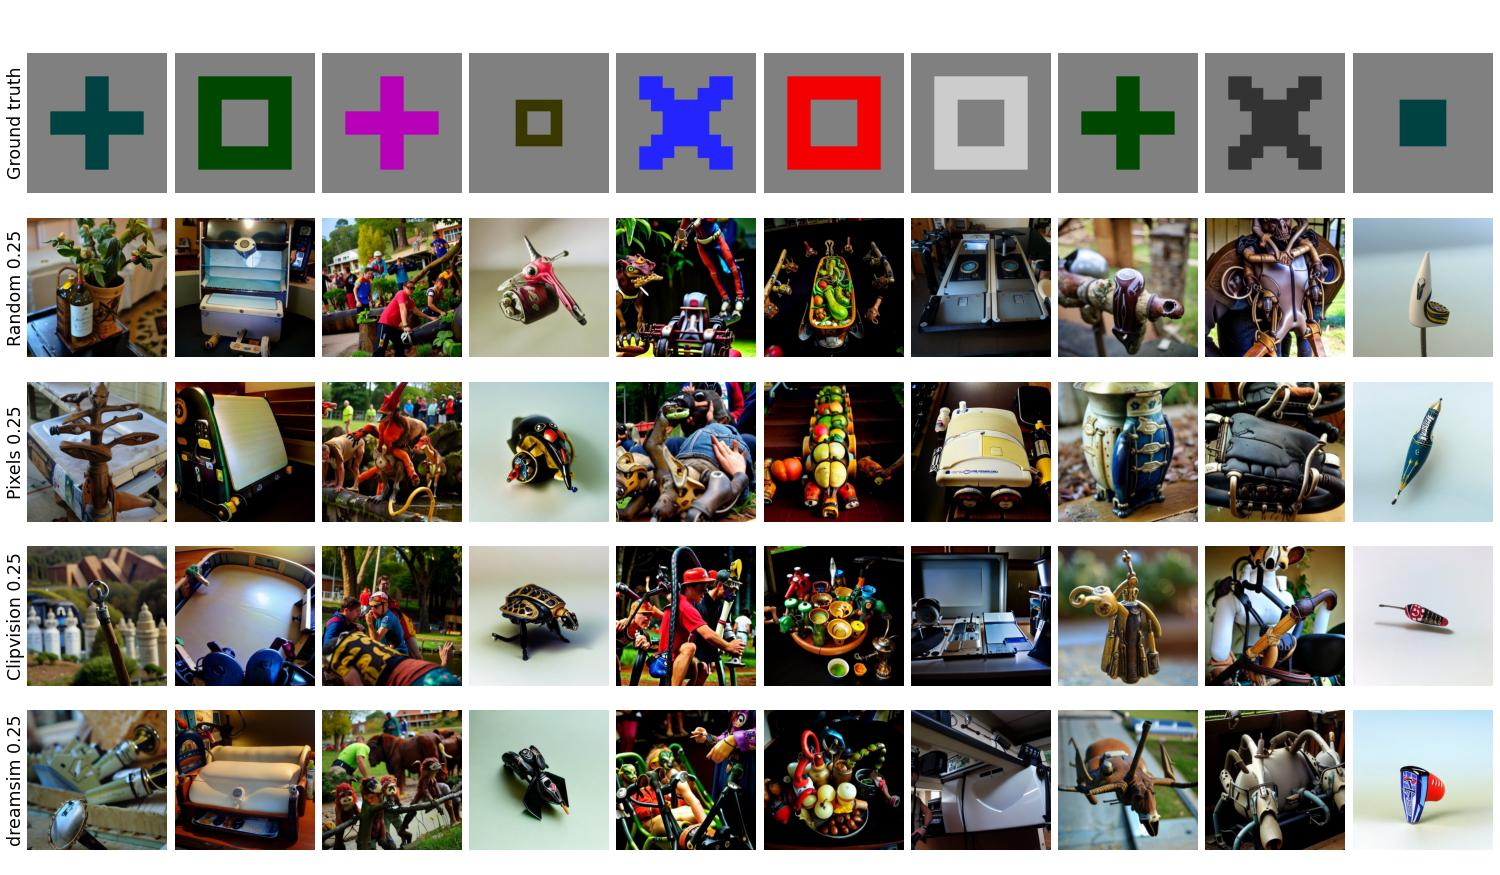
\includegraphics[width=1\textwidth]{plots/dropout_qual_eval_bd_art.JPEG}
   \caption{Qualitative Results for different dropout strategies with the brain-diffuser on artificial shapes}\label{fig:dropout_qual_eval_bd_art}
\end{figure}


\begin{figure}[ht]
   \centering
   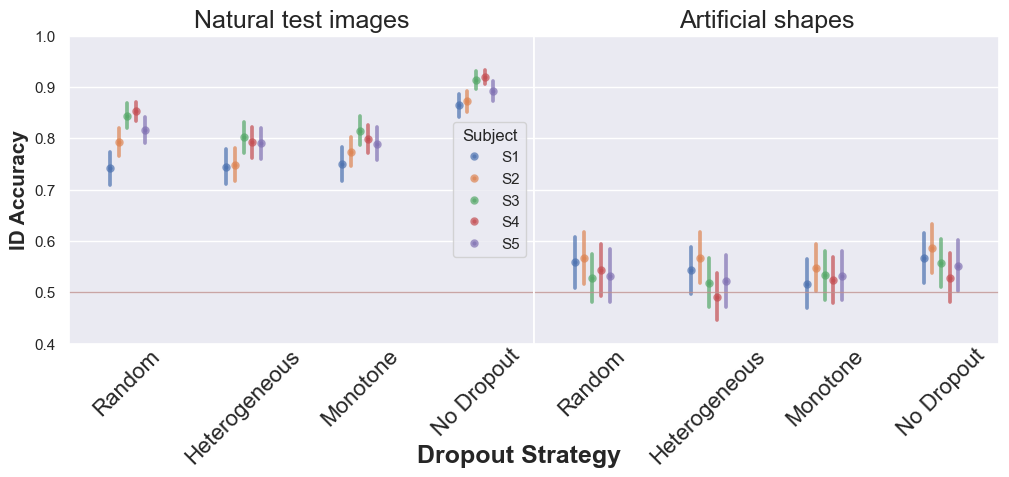
\includegraphics[width=1\textwidth]{plots/dropout_discussion_translator_id_acc_cliptext.png}
   \caption{Cliptext Decoder Results for monotone vs.\ heterogeneous training images}\label{fig:dropout_discussion_translator_id_acc_cliptext}
 \end{figure}
 
 \begin{figure}[ht]
   \centering
   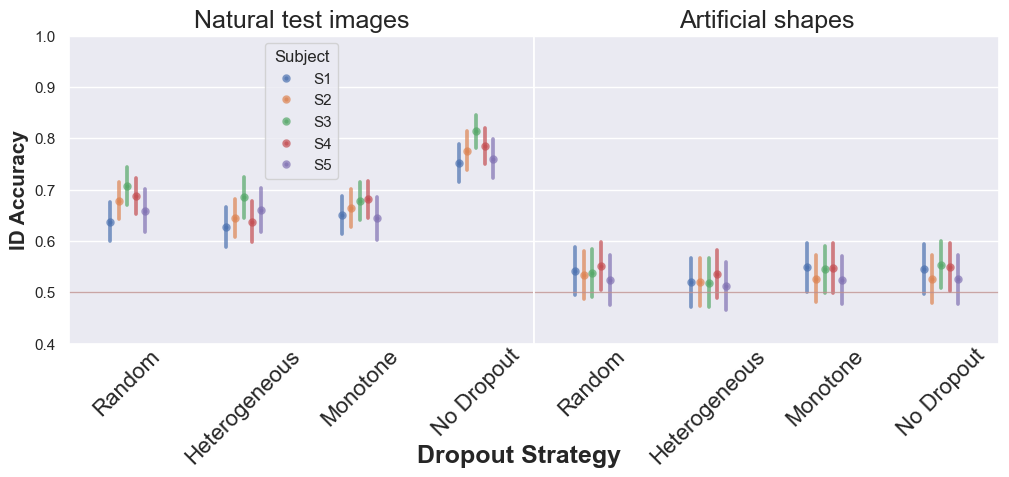
\includegraphics[width=1\textwidth]{plots/dropout_discussion_translator_id_acc_clipvision.png}
   \caption{Clipvision Decoder Results for monotone vs.\ heterogeneous training images}\label{fig:dropout_discussion_translator_id_acc_clipvision}
 \end{figure}
 
 \begin{figure}[ht]
   \centering
   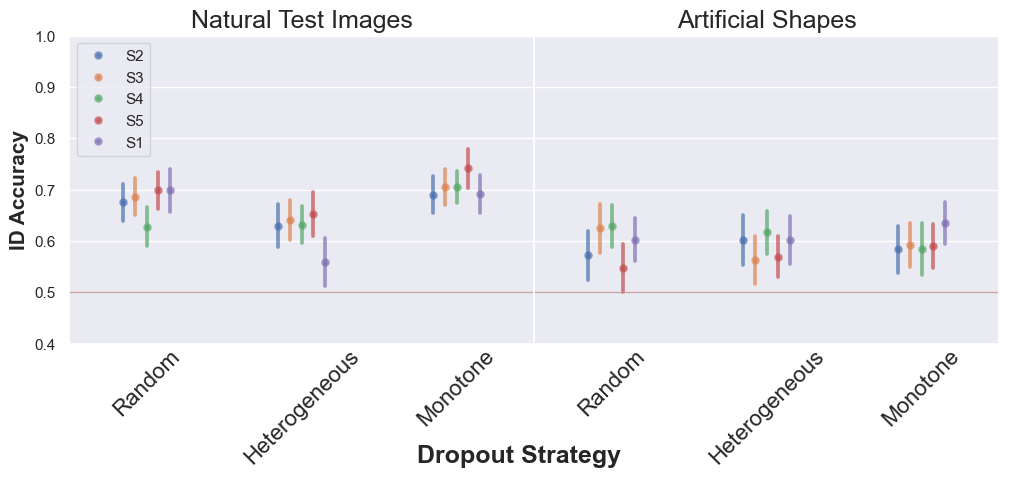
\includegraphics[width=1\textwidth]{plots/dropout_discussion_translator_id_acc_vdvae.png}
   \caption{VDVAE Decoder Results for monotone vs.\ heterogeneous training images}\label{fig:dropout_discussion_translator_id_acc_vdvae}
 \end{figure}
 
 \begin{figure}[ht]
   \centering
   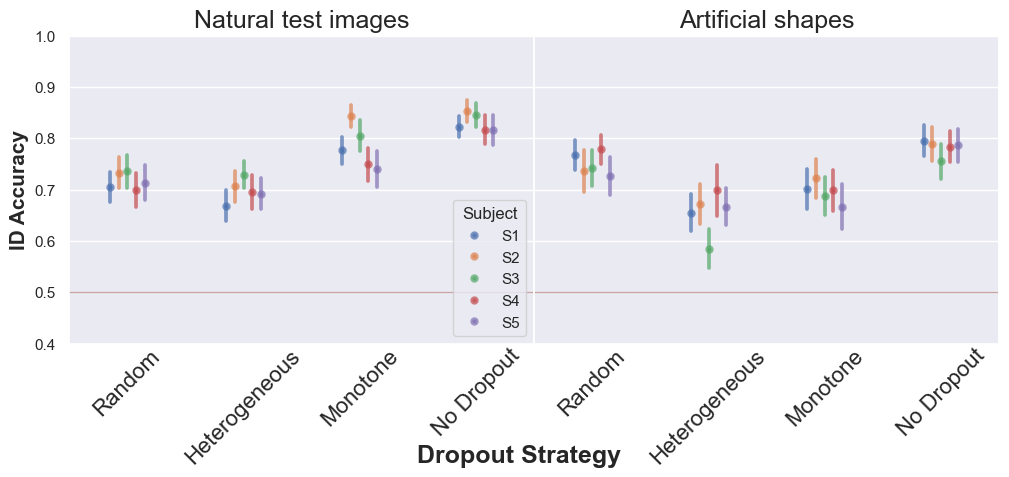
\includegraphics[width=1\textwidth]{plots/dropout_discussion_translator_id_acc_icnn.png}
   \caption{ICNN Decoder Results for monotone vs.\ heterogeneous training images}\label{fig:dropout_discussion_translator_id_acc_icnn}
 \end{figure}
 
 \begin{figure}[ht]
   \centering
   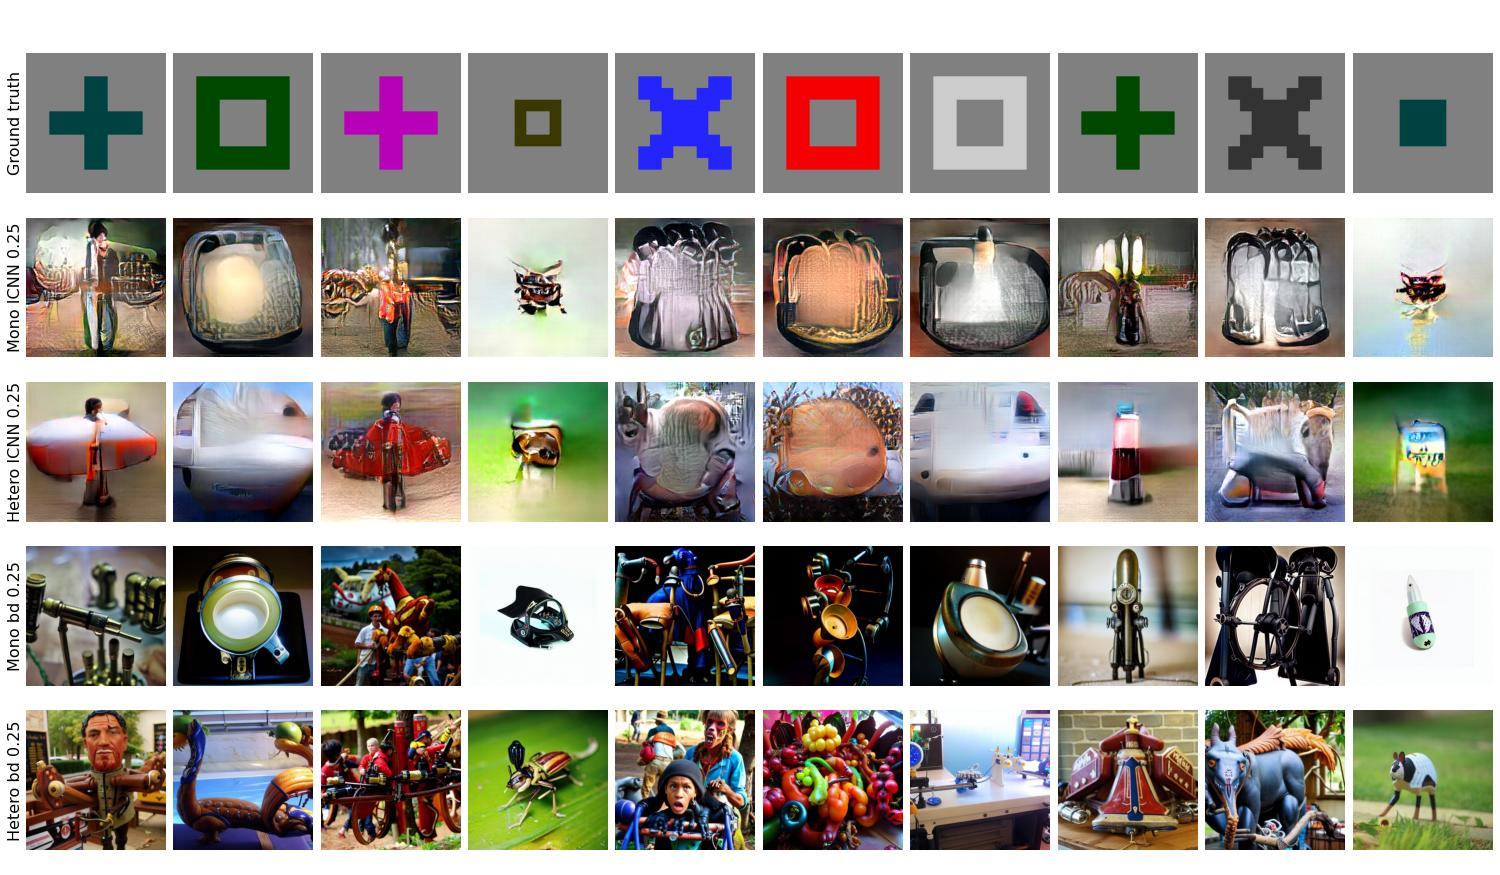
\includegraphics[width=1\textwidth]{plots/dropout_discussion_art.JPEG}
   \caption{Qualitative Results for monotone vs.\ heterogeneous training images on Artificial Shapes}\label{fig:dropout_discussion_art}
 \end{figure}


\section{Ai Captions}

\begin{figure}[ht]
   \centering
   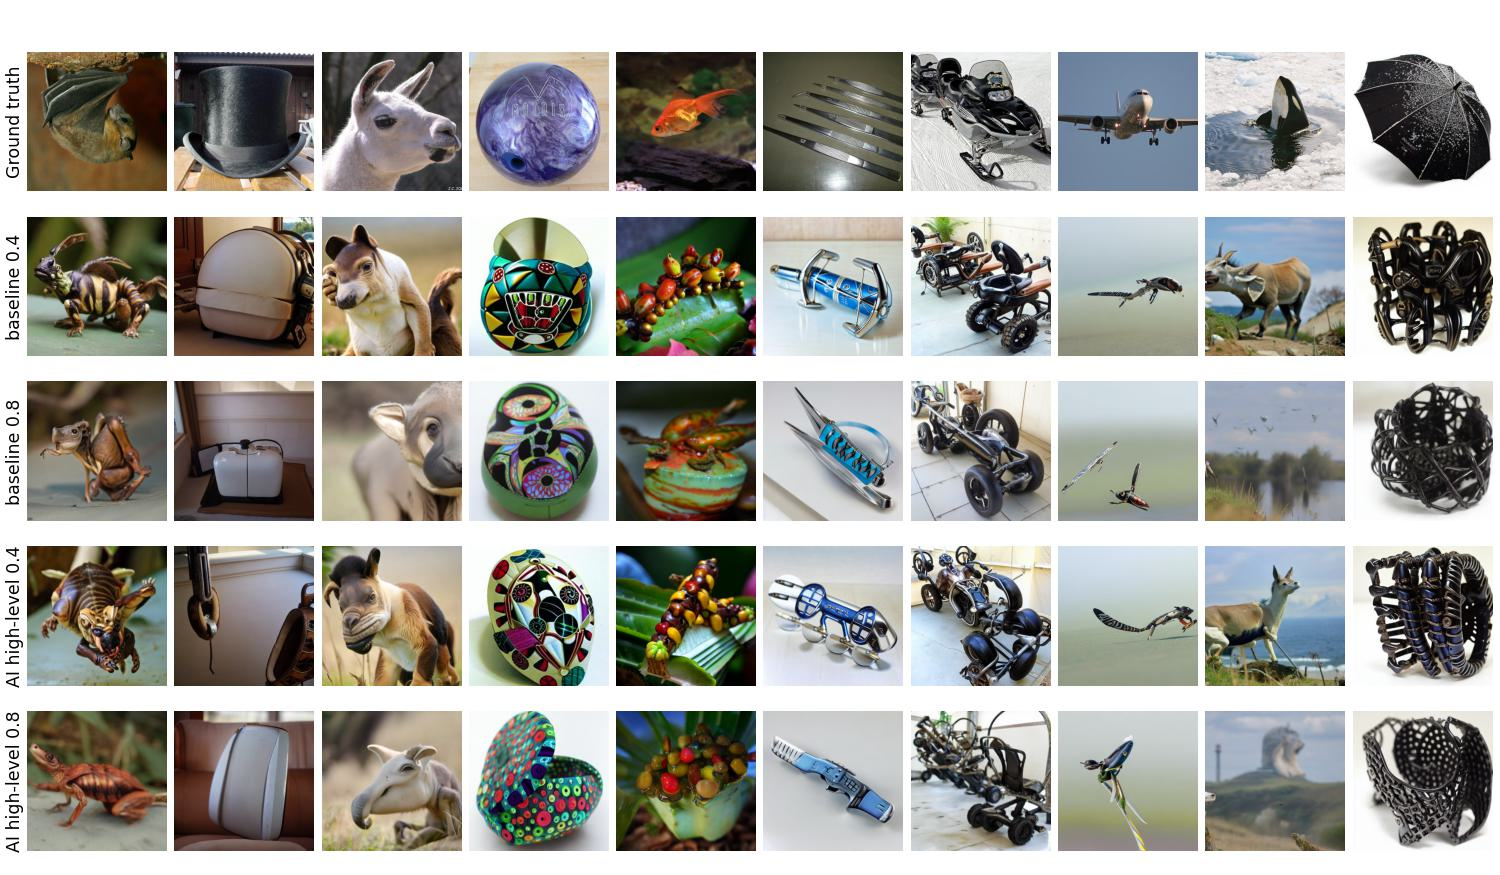
\includegraphics[width=1\textwidth]{plots/aicap_qual_test_highlevel_appendix.JPEG}
   \caption{Qualitative Results for the high-level AI captions on Natural Test Images}\label{fig:aicap_qual_test_highlevel_appendix}
\end{figure}

\begin{figure}[ht]
   \centering
   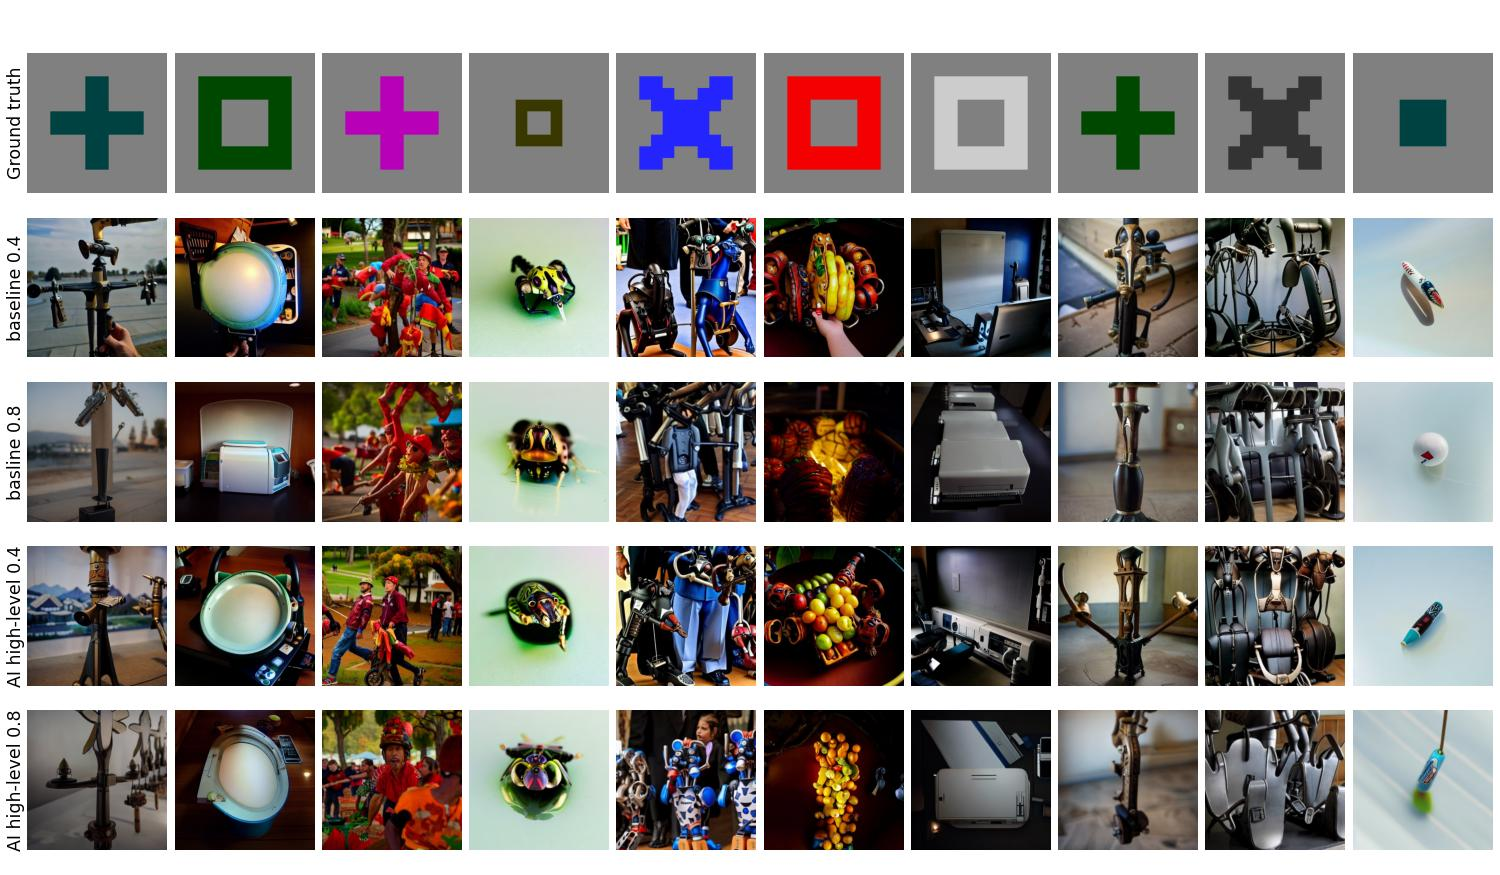
\includegraphics[width=1\textwidth]{plots/aicap_qual_art_highlevel_appendix.JPEG}
   \caption{Qualitative Results for the high-level AI captions on Artificial Shapes}\label{fig:aicap_qual_art_highlevel_appendix}
\end{figure}


\begin{figure}[ht]
   \centering
   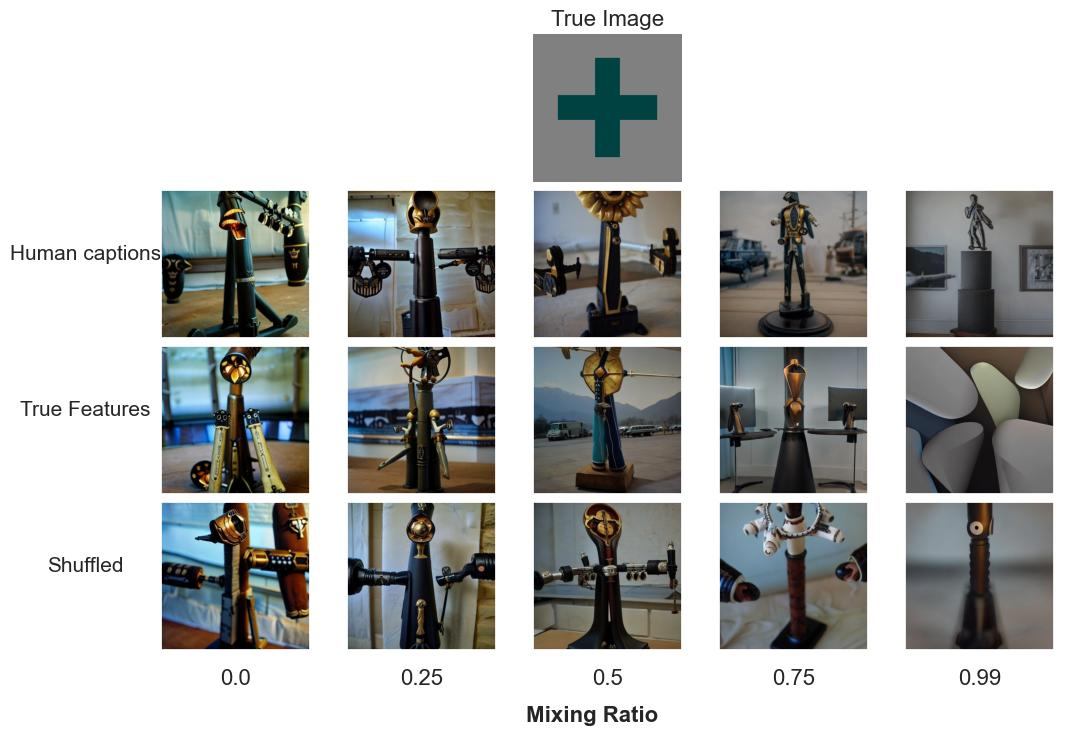
\includegraphics[width=1\textwidth]{plots/aicap_reconstruction_evolution_art_0.JPEG}
   \caption{Qualitative influence of different mixing ratios on Artificial Shapes}\label{fig:aicap_reconstruction_evolution_art_0}
\end{figure}

\begin{figure}[ht]
   \centering
   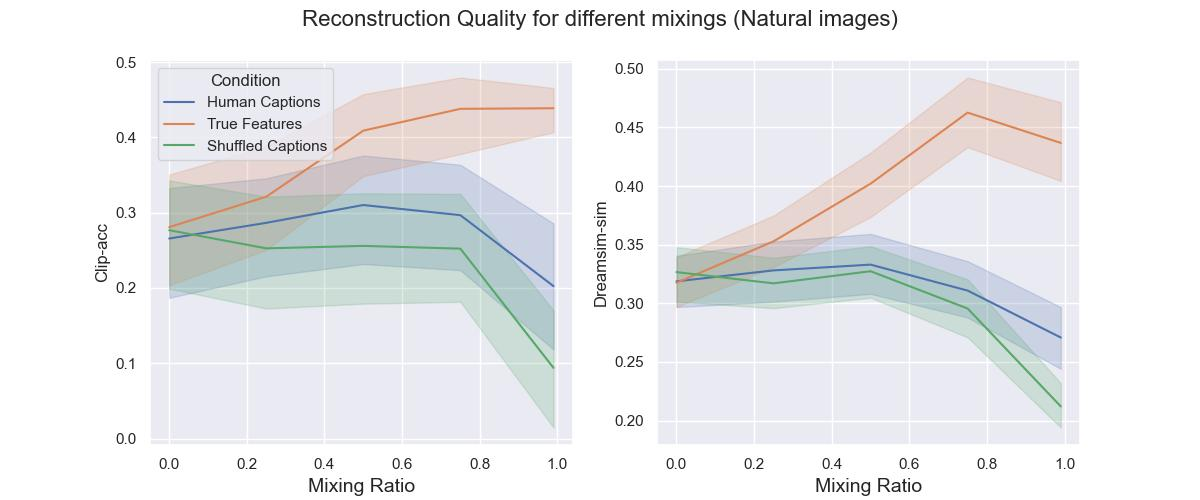
\includegraphics[width=1\textwidth]{plots/aicap_reconstruction_quant_evolution_test.JPEG}
   \caption{Qualitative influence of different mixing ratios on Natural Test Images}\label{fig:aicap_reconstruction_quant_evolution_test}
\end{figure}

\begin{figure}[ht]
   \centering
   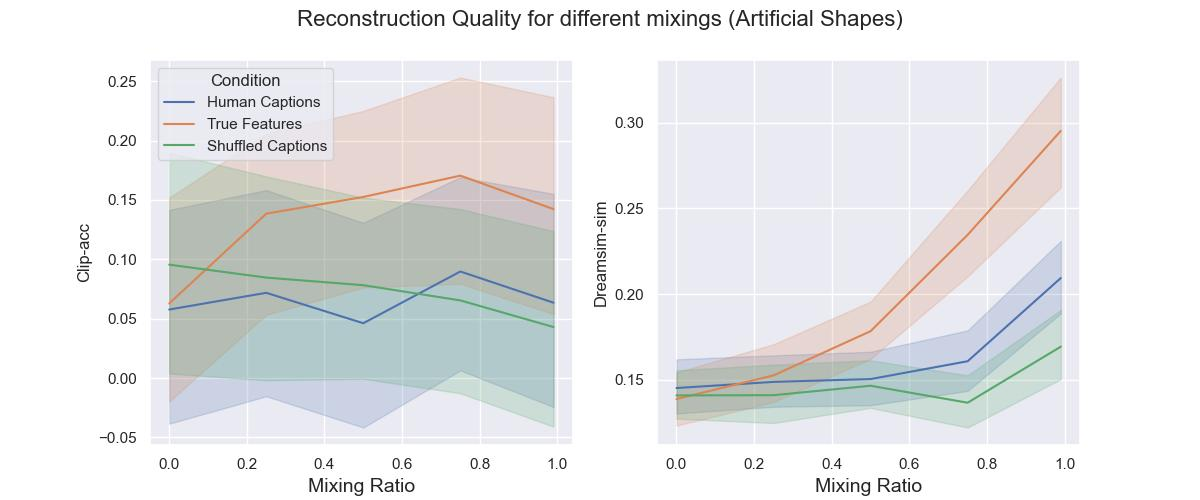
\includegraphics[width=1\textwidth]{plots/aicap_reconstruction_quant_evolution_art.JPEG}
   \caption{Qualitative influence of different mixing ratios on Artificial Shapes}\label{fig:aicap_reconstruction_quant_evolution_art}
\end{figure}

\section{Perturbations}
\begin{figure}[ht]
    \centering
    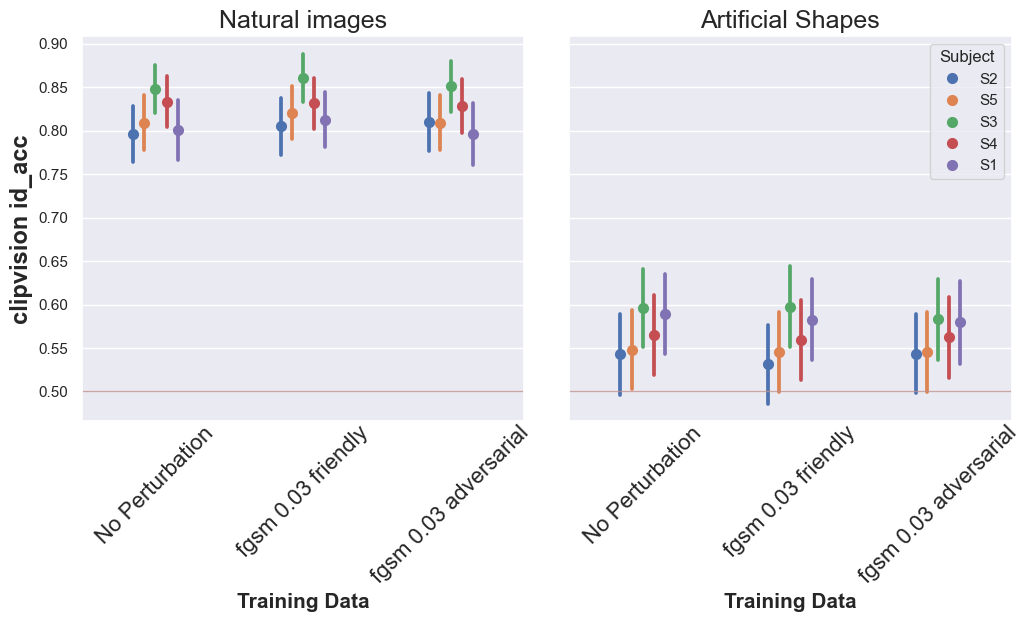
\includegraphics[width=1\textwidth]{plots/advpert_translator_fgsm_0.03.png}
    \caption{FGSM 0.03 Translator Performance}\label{fig:advpert_translator_fgsm_0}
\end{figure}

\begin{figure}[ht]
    \centering
    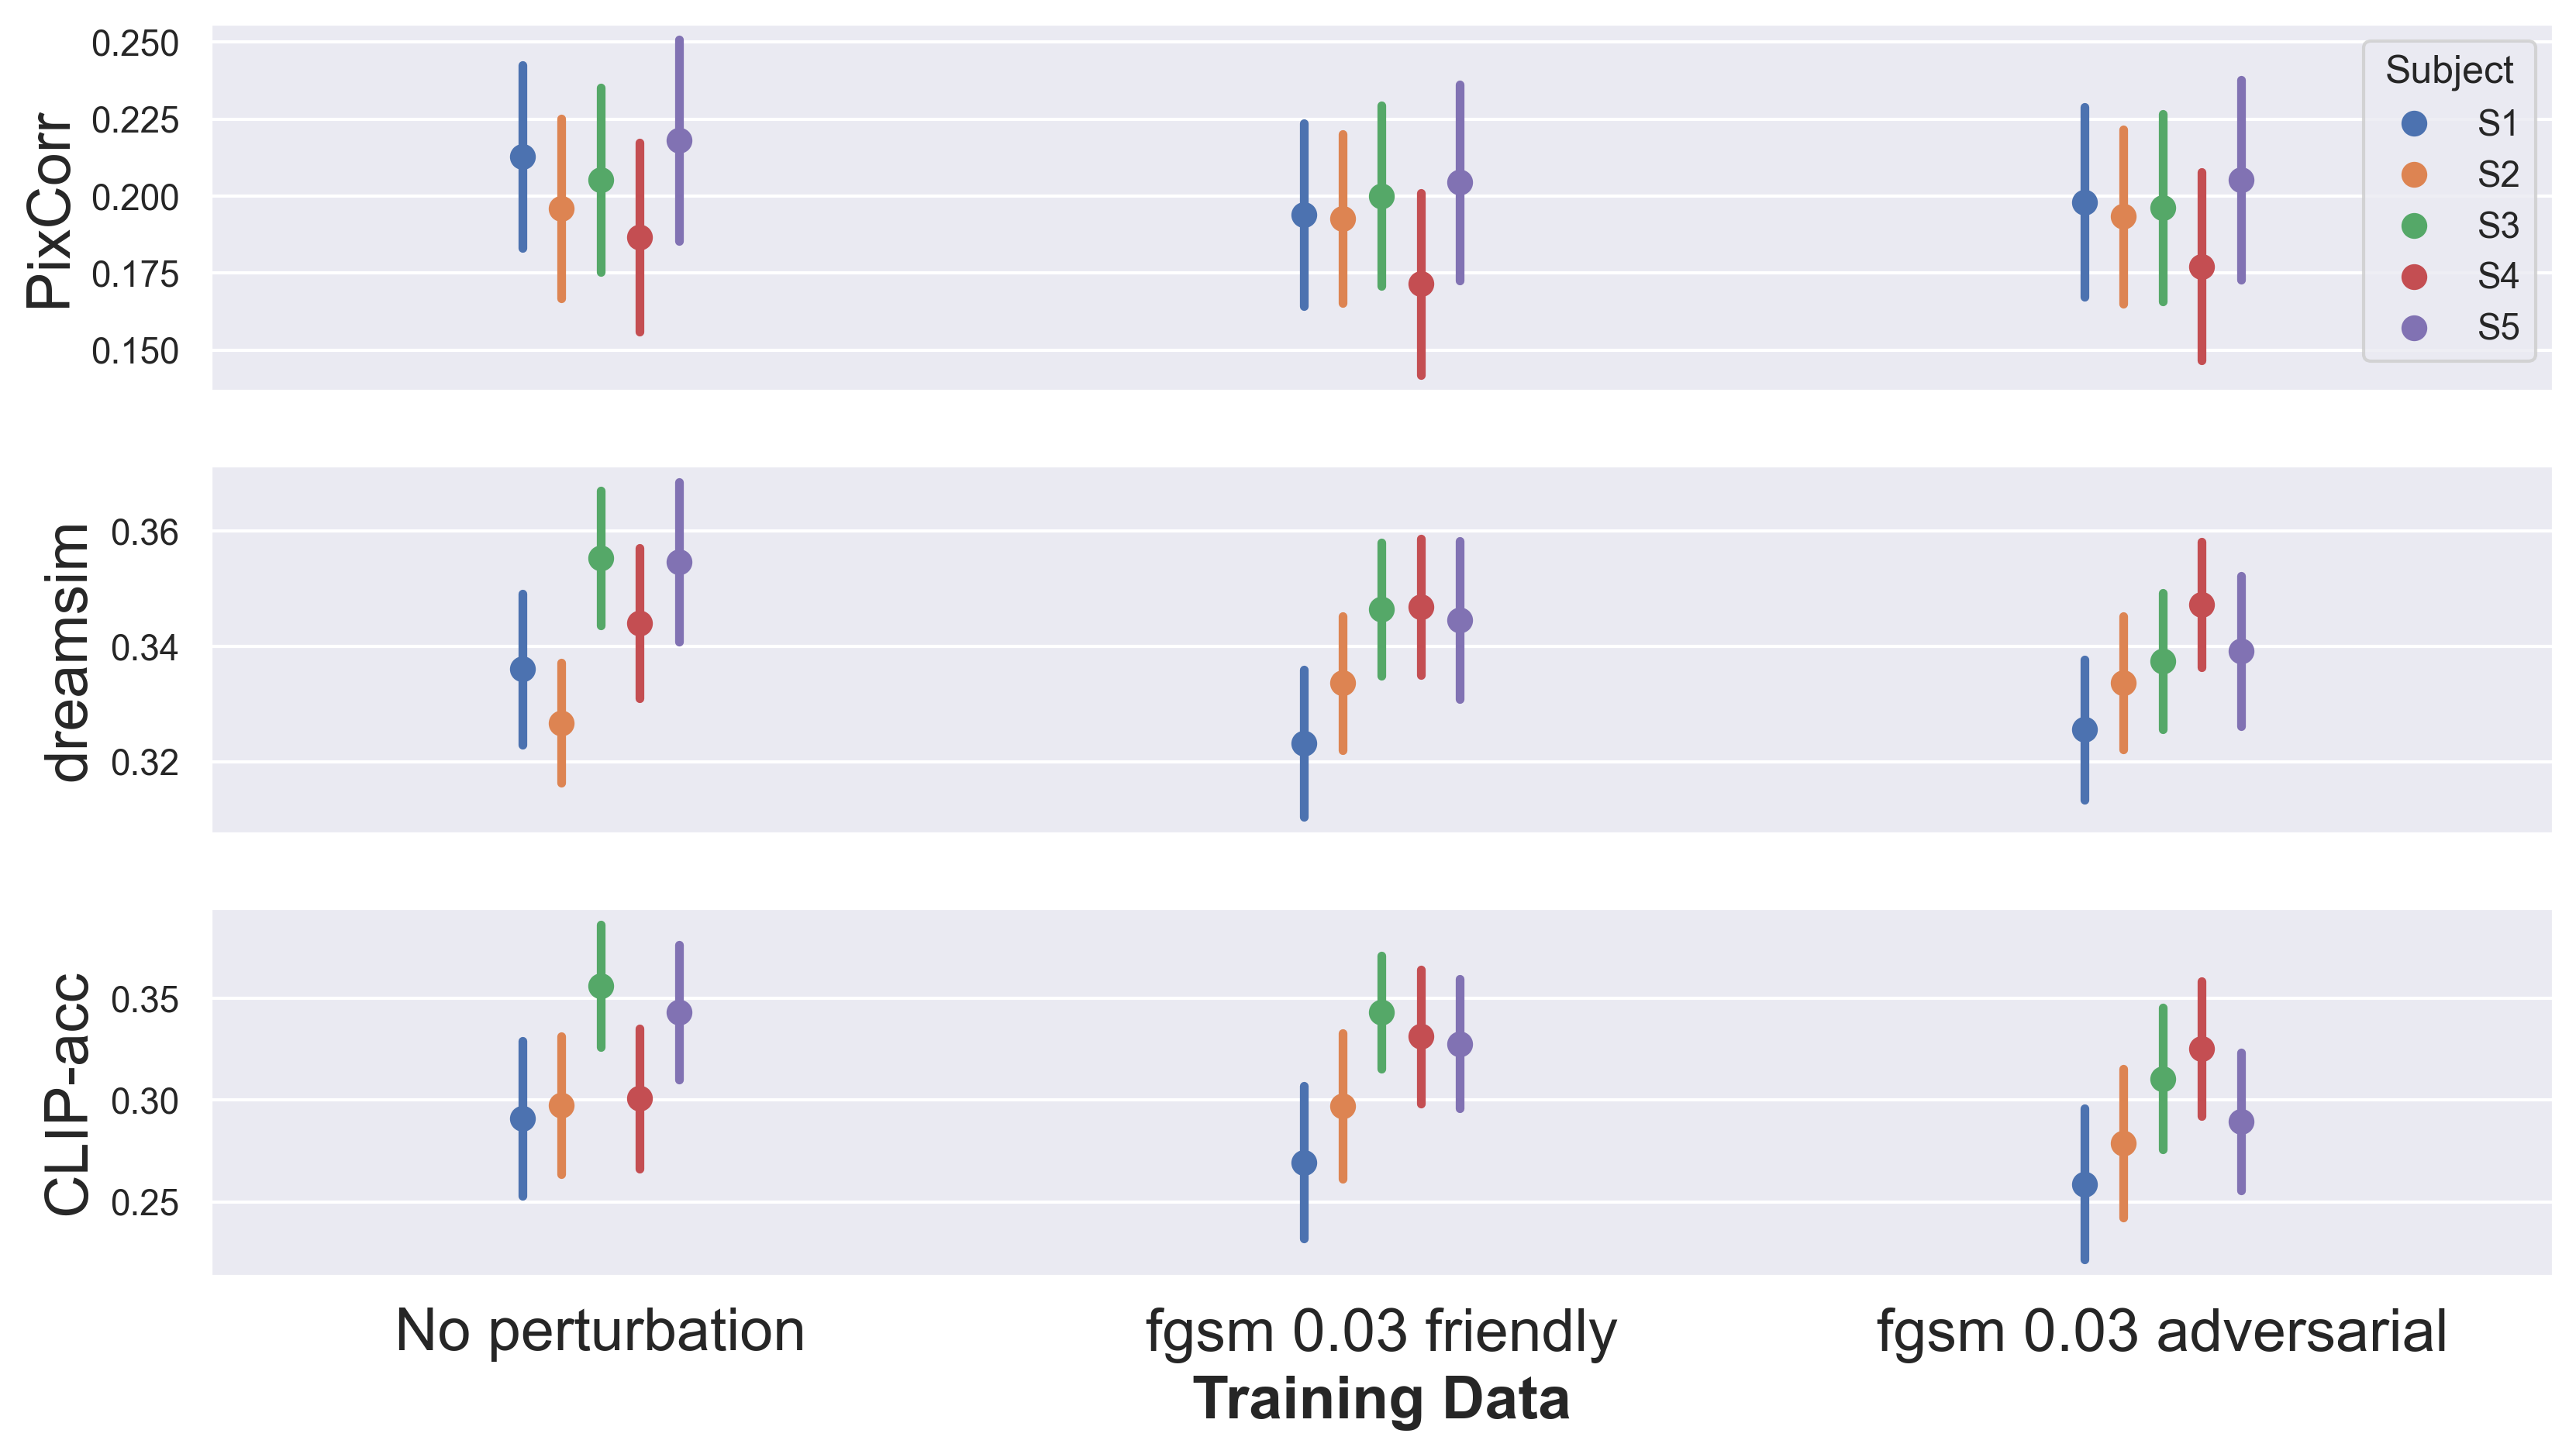
\includegraphics[width=1\textwidth]{plots/advpert_reconstruction_test_fgsm_0.03.png}
    \caption{FGSM 0.03 Reconstruction Performance Natural Test Images}\label{fig:advpert_reconstruction_test_fgsm_0.03}
\end{figure}

\begin{figure}[ht]
    \centering
    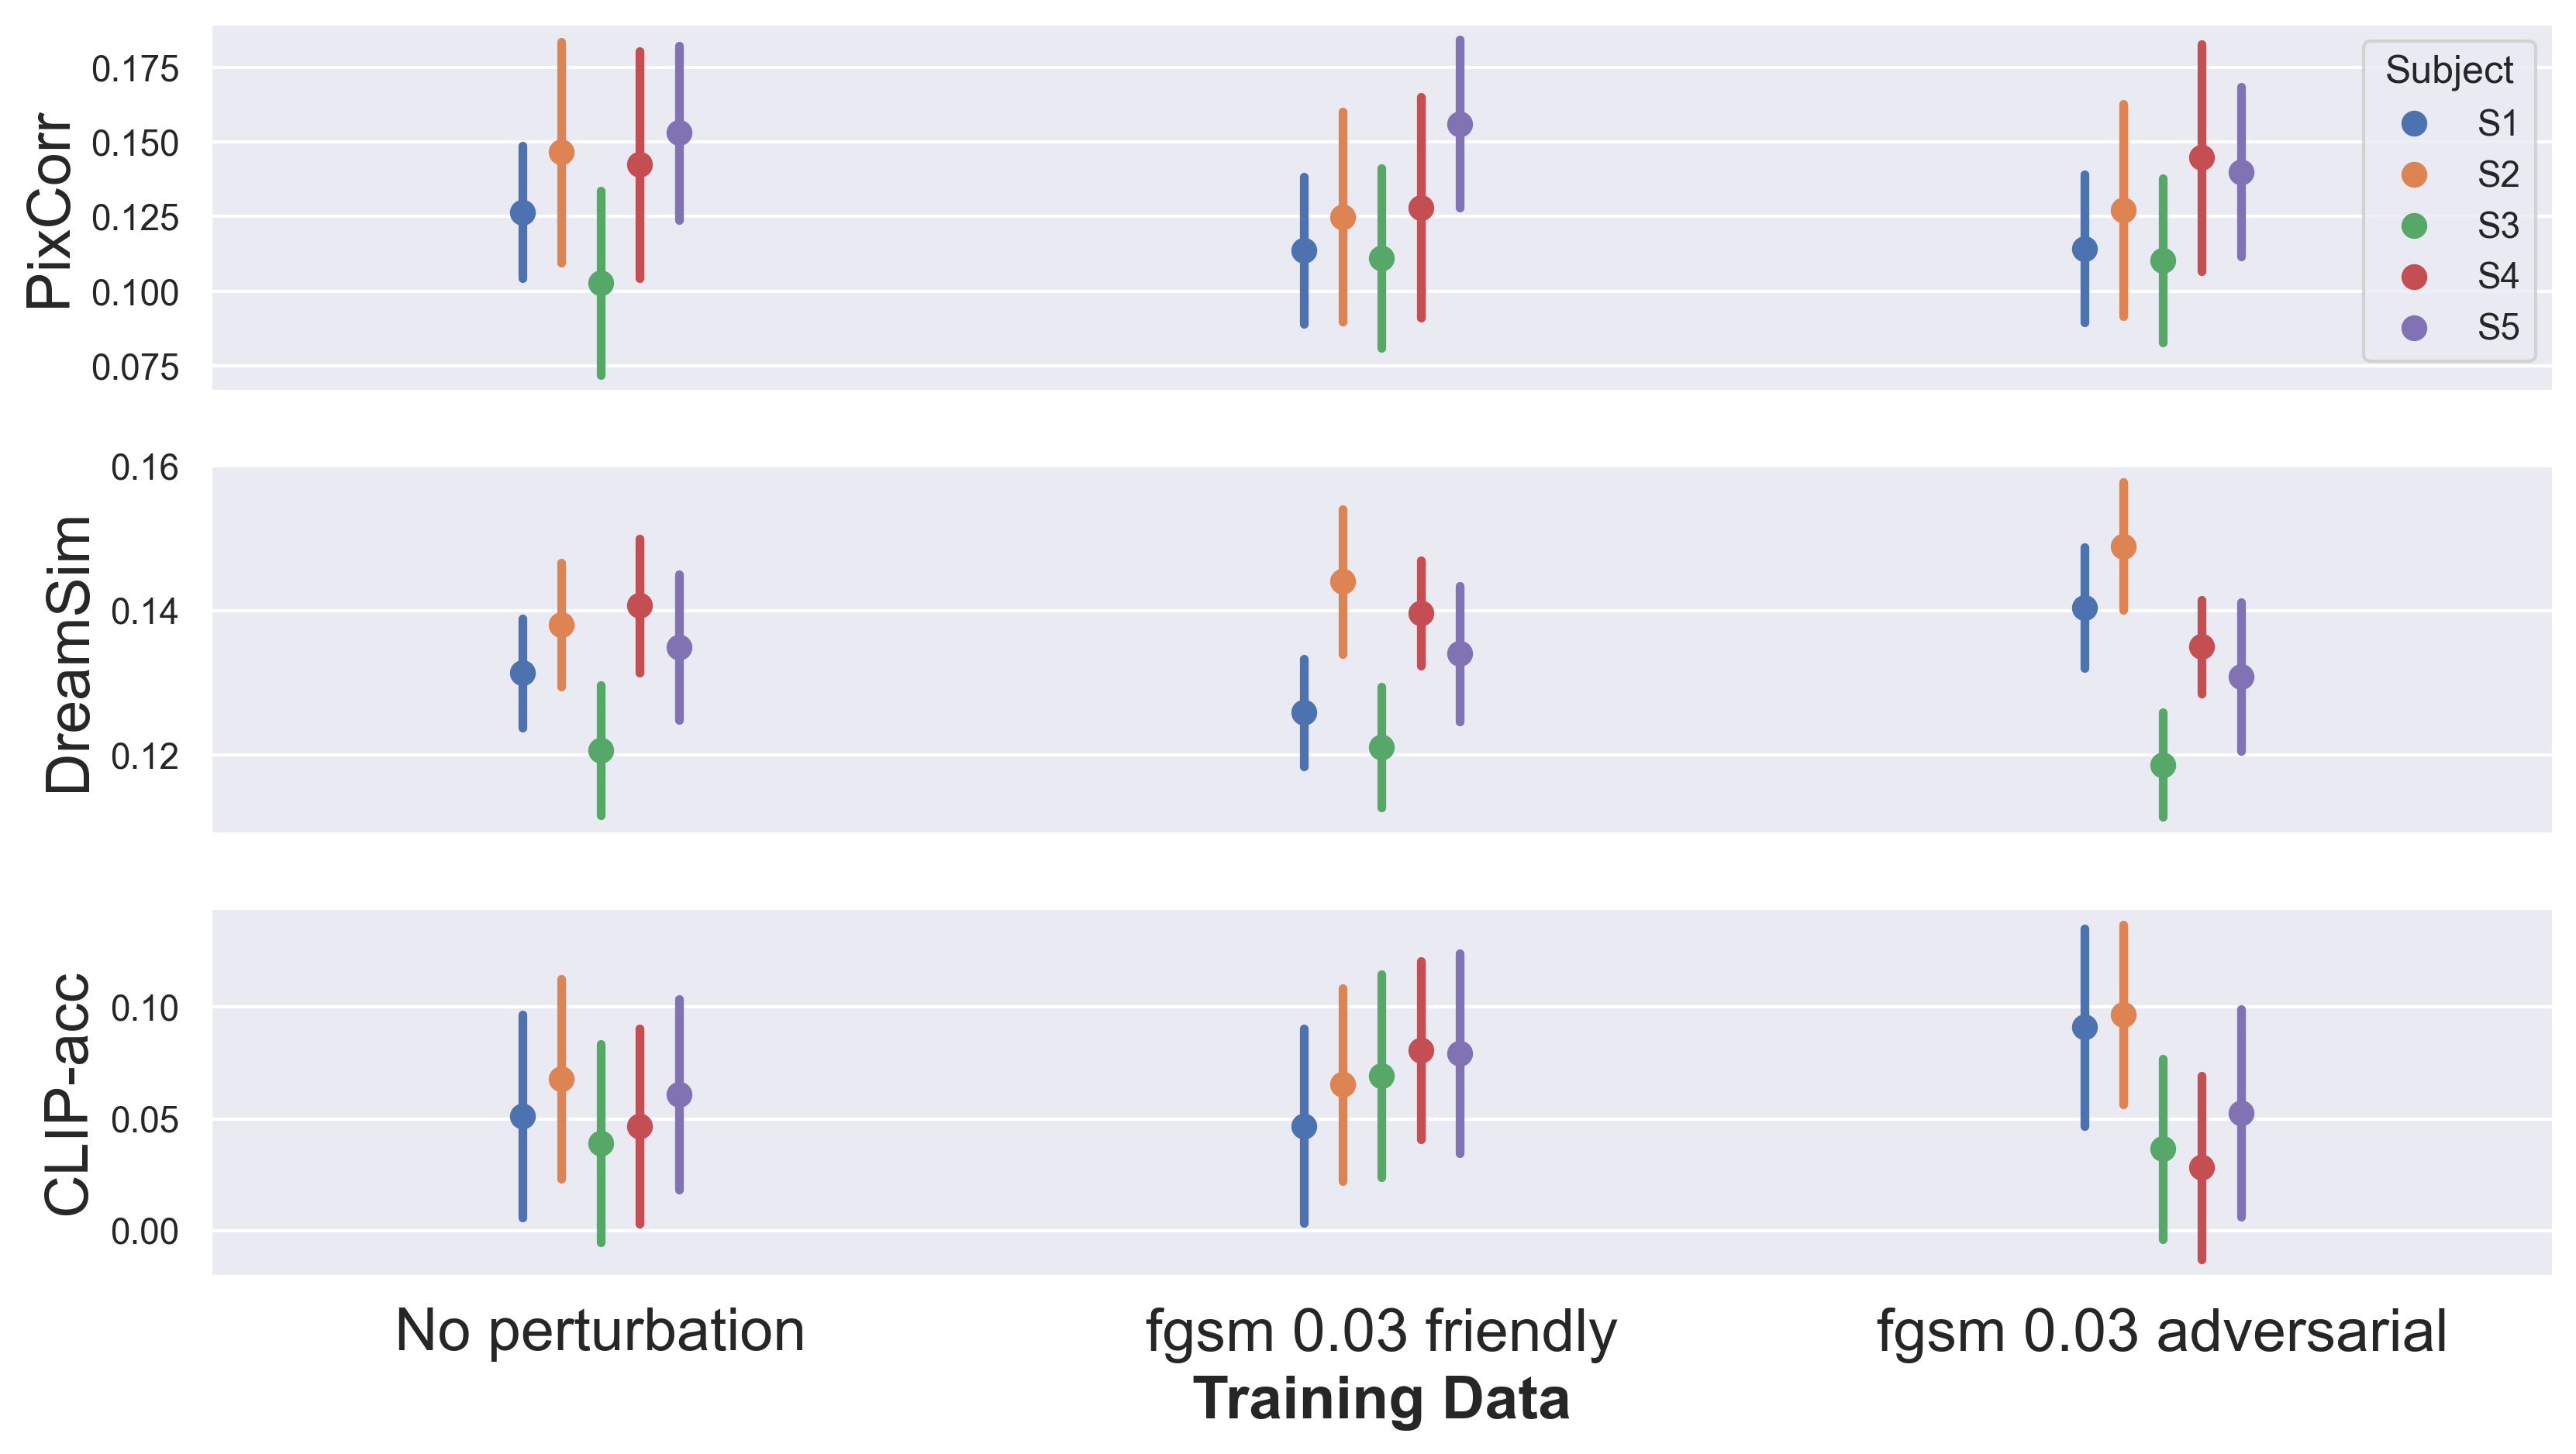
\includegraphics[width=1\textwidth]{plots/advpert_reconstruction_art_fgsm_0.03.png}
    \caption{FGSM 0.03 Reconstruction Performance Artificial Shapes}\label{fig:advpert_reconstruction_art_fgsm_0.03}
\end{figure}

\begin{figure}[ht]
   \centering
   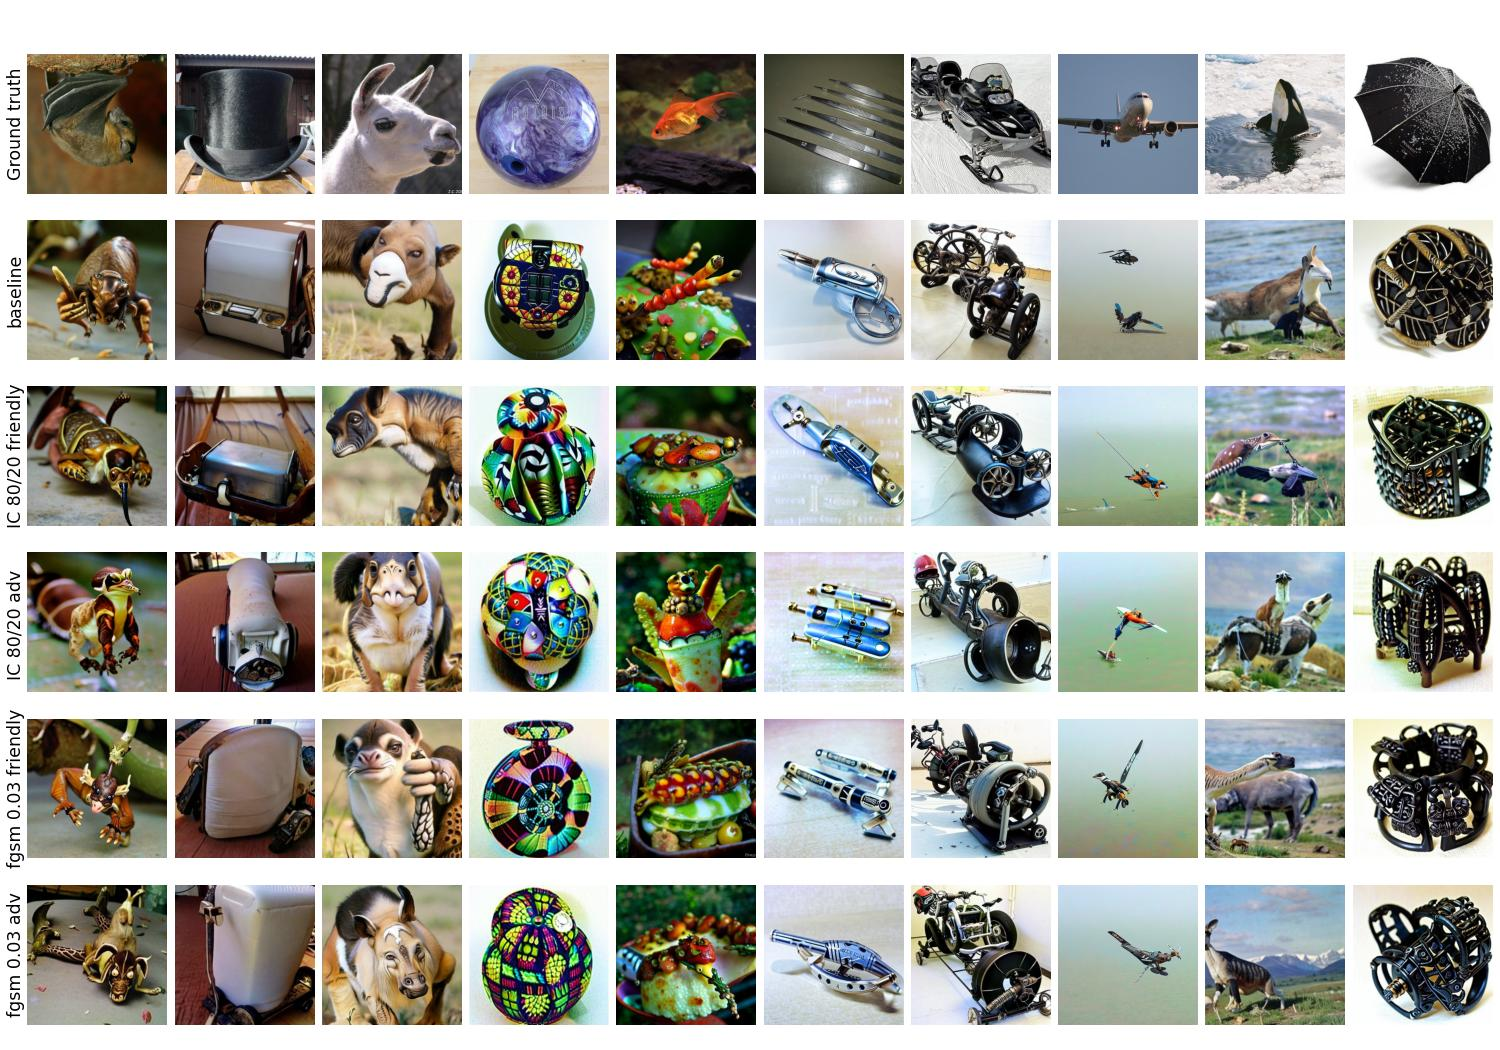
\includegraphics[width=1\textwidth]{plots/advpert_qual_test.JPEG}
   \caption{Qualitative Results for the perturbations experiment Natural Test Images}\label{fig:advpert_qual_test}
\end{figure}

\begin{figure}[ht]
   \centering
   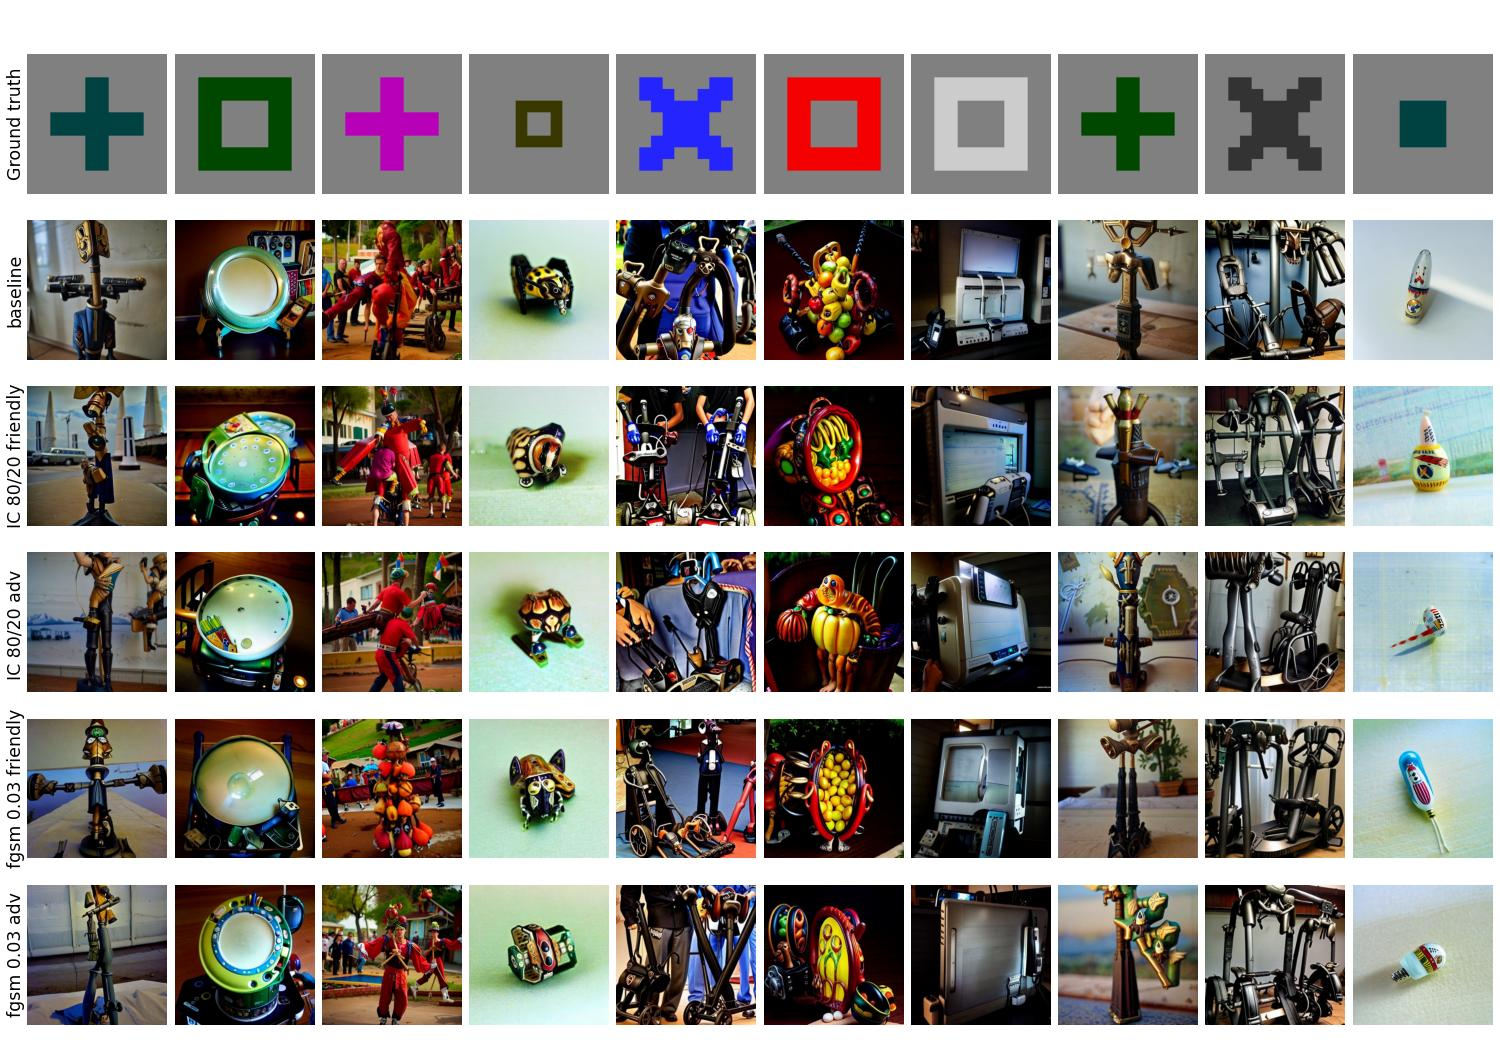
\includegraphics[width=1\textwidth]{plots/advpert_qual_art.JPEG}
   \caption{Qualitative Results for the perturbations experiment Artificial Shapes}\label{fig:advpert_qual_art}
\end{figure}

